\documentclass[journal]{IEEEtran}
\usepackage{cite}
\usepackage[pdftex]{graphicx}
\usepackage[cmex10]{amsmath}
\usepackage{amssymb}
\interdisplaylinepenalty=2500
\usepackage{array}
\usepackage{dblfloatfix}

%%%Undefined packages
\usepackage{todonotes}
\usepackage{changes}
\definechangesauthor[name={Min Tan} color=orange]{MT}

\begin{document}
\title{A Single-Control-Circuit Multiple-Output Digital Low Dropout Regulator With Delay Switching}
\author{
        Kaixuan~Ye,~\IEEEmembership{Student Member,~IEEE,}
        Min~Tan,~\IEEEmembership{Member,~IEEE,}% <-this % stops a space
\thanks{The authors are with the School of Optical and Electronic Information,
Huazhong University of Science and Technology, Wuhan 430074, China (email:
mtan@hust.edu.cn).}
        }

\markboth{Journal of \LaTeX\ Class Files,~Vol.~14, No.~8, August~2015}%
{K.~Ye\MakeLowercase{\textit{et al.}}: DLDO Paper Draft}


\maketitle

\begin{abstract}
This paper presents a novel single-control-circuit multiple-output digital low dropout regulator (DLDO). Operating in the time division multiplexing mode, this DLDO can share a single control circuit and regulate multiple outputs at different time period. With the proposed delay switching technique, the cross regulation between different outputs can be totally eliminated. A prototype with two outputs was fabricated with UMC 130nm process and this approach can be extended to more outputs theoretically. As the DLDO design becomes more and more complicate and the control circuit takes up more and more area, this design points out a very promising way to save the total chip area.\\

\begin{IEEEkeywords}
Delay switching, time-division multiplexing, digital low dropout regulator.
\end{IEEEkeywords}
\end{abstract}

\section{Introduction}
In today's System on Chip (SoC) design, it usually requires multiple power domains to obtain the maximum energy efficiency for different application demands \cite{original,AALDO,AALDO1,coarse-fine,pipeline,asynchrounous,recursive}. To get a highly-efficient, highly-accurate power domain, the most popular choice is to apply the hierarchical power managing network. A basic hierarchical power managing network is depicted in Fig.\ref{hierarchical}. Firstly, the DC-DC buck converters scale down the battery voltage to the operating voltage of the application with high efficiency. Then, a post regulator, most frequently a low dropout regulator (LDO), is connected with the DC-DC to reduce the output voltage ripple. Finally, the fine-grained voltage is supplied for different function units such as RFs, AD/DAC, I/Os in the circuit.

Traditionally, the LDOs are analog circuits which are implemented with error amplifiers and power stages. However, with the SoC supply voltage constantly scaling down, it becomes harder and harder for the amplifiers to meet the performance requirements. And LDO implemented with digital logics, or DLDO, draws great attention in academic recently. The DLDO was first proposed in \cite{original}. It consists of a clocked comparator, a bidirectional shift register and a PMOS array. The comparator compares the output with the reference. When the output is below the reference, the shift register shift right and turn on a unit of the PMOS array at every clock rising edge or vice versa. When the current provided by the PMOS array meet the load current, the output is regulated to the around of the reference.

However, the original DLDO suffer from large drop voltage and ripple. And many advanced techniques have been proposed to address these problems. In\cite{coarse-fine}, two MOS arrays with different size are employed. In steady state, the small MOS array is connected to the loop, and it switches to the large MOS array when the load changes. As a result, a relatively small drop voltage and ripple is realized simultaneously. In \cite{AALDO,NANDbasedAAloop}, an analog-assisted (AA) loop composing of coupling capacitor and resistor is added. The AA loop sense the output undershoot and feed it back to the buffer of the PMOS array. Consequently, the PMOS array can response to the output before the clock rising edge, so greatly reduce the undershoot. In \cite{pipeline}, it adopts a pipeline control structure and a 3-D power stage to realize the multi-step switching scheme. As a result it speeds up the transient response while maintaining a small output voltage ripple. And in \cite{recursive}, it proposed a recursive DLDO which improves the performances by applying a SAR-like binary search algorithm and a sub-LSB pulse width modulation duty control scheme. 
\begin{figure}[t!]
    \centering
    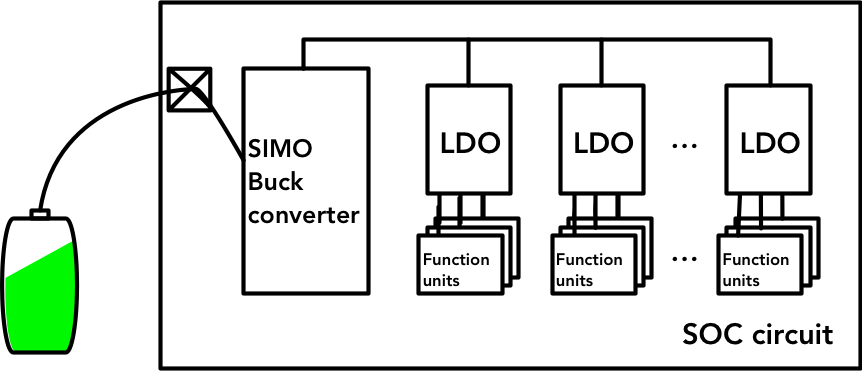
\includegraphics{pic/DLDOsche/SOCcircuit.pdf}
    \caption{Hierarchical power managing network in SoC}
    \label{hierarchical}
\end{figure}

Although all these techniques are effective in some way, with the control circuit becoming more and more complicated, the area took up by the control circuit become equivalent and even greater than the power stage. So it becomes a very interesting topic how we can improve the area efficiency of the control circuit. To improve chip area efficiency, the time-division-multiplexing (TDM) scheme has been applied in many other circuits and has achieved great success. As is a digital concept, this scheme should be available to the DLDO design as well.

The remainder of this paper is organized as follow. In section II, we discuss the TDM scheme in other circuit, and address a method to apply it to DLDO. In section III, we present the architecture and working principles of the proposed TDM DLDO design. In section IV, we interpret the circuit implementation and design considerations. In section V, we show the measurement results along with comparisons. In section VI, we conclude our proposed design.
%%This paragragh needs further tuning.
\section{TDM scheme}
In some circuit designs, a certain building block takes up a great percentage of the whole chip area. Instances are like the controller in the micro ring modulator, the inductor in the DC-DC converter, and the compensation capacitor in the low dropout regulator (LDO). Normally, more than one such circuits are needed in a SoC circuit, and the most straightforward way to realize it is to implement N single output such circuits. However, one the one hand, this immoderately consumes the chip area, and on the other hand, passive devices like inductor and capacitor may bring about great noise to the circuit. To solve this problem, the TDM scheme has been applied to many circuits and have achieved great success.
\subsection{TDM micro ring modulator}
In the burgeoning integrated optoelectronic design, the silicon Micro Ring Modulator (MRM) is believed to be the most important device to realize optical interconnect, which have been proposed to displace electrical interconnects as the next generation I/O links due to its ultra-wide bandwidth and low loss advantages \cite{wangzhicheng}. However, as is highly sensitive to the thermal fluctuation, the MRM usually requires a feedback control circuit to stabilize its resonant wavelength. Normally, the control circuit is much larger than the micro ring, and in order to save chip area, \cite{wangzhicheng} have proposed a TDM scheme to simultaneous lock the wavelength of multiple silicon micro rings.
\begin{figure}[t!]
    \centering
    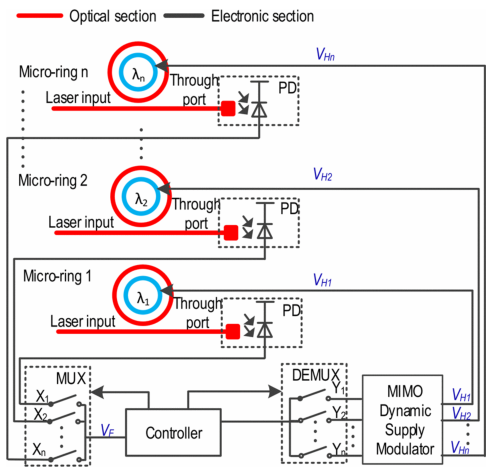
\includegraphics[width=\linewidth]{pic/TDM/MRM.pdf}
    \caption{The TDM scheme applying in micro ring design}
    \label{fig:MRM}
\end{figure}

Fig.\ref{fig:MRM} shows the working principle of the TDM scheme. The MUX and DEMUX connect the photo detector(PD) and its corresponding supply modulator to the controller at different time intervals, as a result, the shared controller, which is composed of an ADC, a MCU and a DAC, can cope with the information of different micro rings at different time period.

\subsection{SIMO DC-DC Converter}
\begin{figure}[t!]
    \centering
    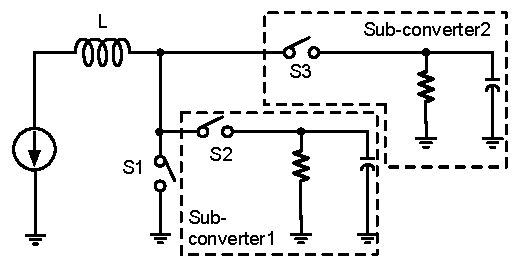
\includegraphics[width=\linewidth]{pic/TDM/DCDC.pdf}
    \caption{The TDM scheme applying in DC-DC converter}
    \label{fig:DCDC}
\end{figure}
\begin{figure}[t!]
    \centering
    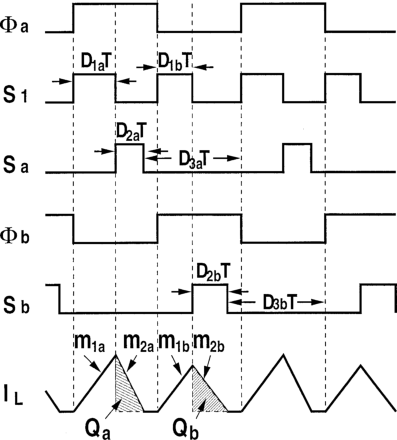
\includegraphics[width=0.8\linewidth]{pic/TDM/DCDC-timing.pdf}
    \caption{Timing diagram of the SIMO DC-DC converter}
    \label{fig:DCDC-timing}
\end{figure}
The DC-DC converters are usually applied in the SoC power management circuit for its high converting efficiency. However an off-chip inductor is required for every DC-DC converter. When multiple power domains exists, which is quite normal in a SoC circuit, multiple DC-DC converters are implemented conventionally. This not only increase the number of required on-chip pads, but also may bring about great noise to the circuit. In \cite{SIMODCDC} an single inductor multiple output (SIMO) DC-DC buck converter is proposed, as is shown in Fig\ref{fig:DCDC}.

Both sub-converter a and converter b are operating in DCM mode, and Fig\ref{fig:DCDC-timing} explicitly interprets the working principle. $\Phi a$ and $\Phi b$ are two complementary phase signals which indicate the regulating period. When $\Phi a = 1$, the sub-converter A is connected to the inductor, and the current through the inductor ramps up at $D_{1a}T$ and ramp down at $D_{2a}T$. Similar current behavior happens again when $\Phi b =1$, and the current is assigned to different sub-converters without affecting each other. 

\subsection{the proposed TDM DLDO}
\begin{figure}[t!]
    \centering
    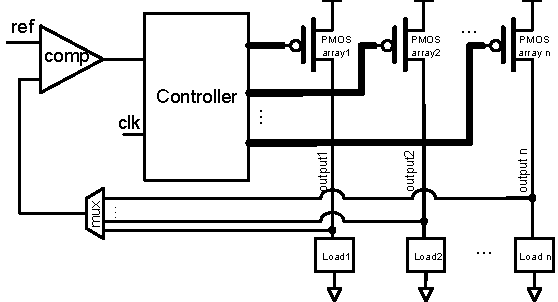
\includegraphics[width=\linewidth]{pic/TDM/TDMDLDO.pdf}
    \caption{the proposed TDM DLDO}
    \label{fig:TDMDLDO}
\end{figure}
Contrary to the analog counterpart, in the Digital LDO design, the control circuit takes up a great percentage of the whole chip area, even greater than the power stage. The control circuit is usually composed of shift registers, and each power MOS array unit needs a shift register stage. So it would be very promising if we can share the control circuit between different outputs like the TDM MRMs and the SIMO DC-DC converters.

Fig.\ref{fig:TDMDLDO} shows our proposed TDM DLDO, and the working principle is very simple and similar to the TDM MRM. The mux select different outputs to the comparator at certain time periods. Then the comparator compares the output voltages with the reference, and the comparison result serves as the input signal of the controller, which finally determines the states of the power PMOS array. Multiple outputs share the single control circuit at different time period, so the proposed DLDO is operating at TDM mode.

\section{Architecture and working principle of the proposed TDM DLDO}
\subsection{Architecture}
The architecture of the proposed TDM DLDO is shown in Fig.\ref{fig:TDMDLDO}. It mainly composes of a comparator, a output MUX, an analog-assisted loop, two groups of latches, namely lat\_0 and lat\_1 in the diagram, two groups of PMOS arrays, in each group the size of the ``coarse'' PMOS array unit is 9 times larger than that of the ``fine'' PMOS array unit, and two groups of shift register, which are coarse and fine shift registers. The shift registers determine the states of the PMOS arrays and can be asynchronously set/reset by the special set/reset block.  

In the whole diagram, not only the comparator, but also the analog-assisted loop and the coarse and fine shift registers are shared the by two outputs. The latches serve as the buffer stage, which also exist in many other DLDO designs\cite{AALDO,AALDO1}. Apart from that, only an additional multiplexer, the ``outputMux'' is added to the circuit, which scarcely bring any additional area to the whole chip. In other word, we almost double the efficiency of the control circuit in terms of area.
\subsection{Delay switching technique}
\begin{figure}[t!]
    \centering
    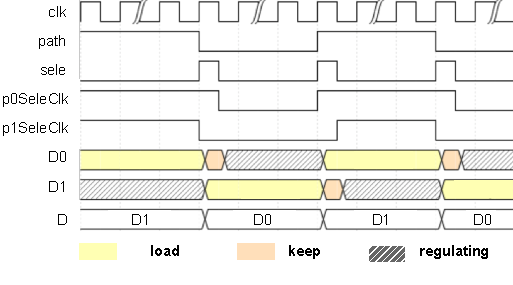
\includegraphics[width=\linewidth]{pic/struc/timing.pdf}
    \caption{Timing diagram of the proposed design}
    \label{fig:timing}
\end{figure}
\begin{figure}[t!]
    \centering
    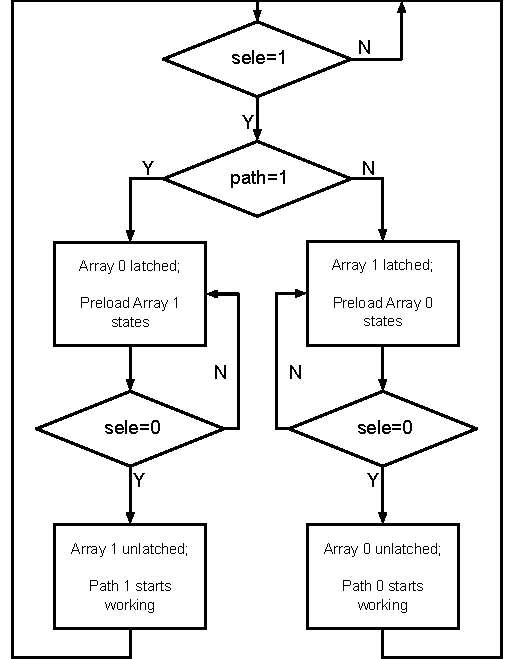
\includegraphics[width=0.9\linewidth]{pic/struc/flowChart.pdf}
    \caption{Flowchart of the delay switching process}
    \label{fig:flowchart}
\end{figure}
\begin{figure*}[t!]
    \centering
    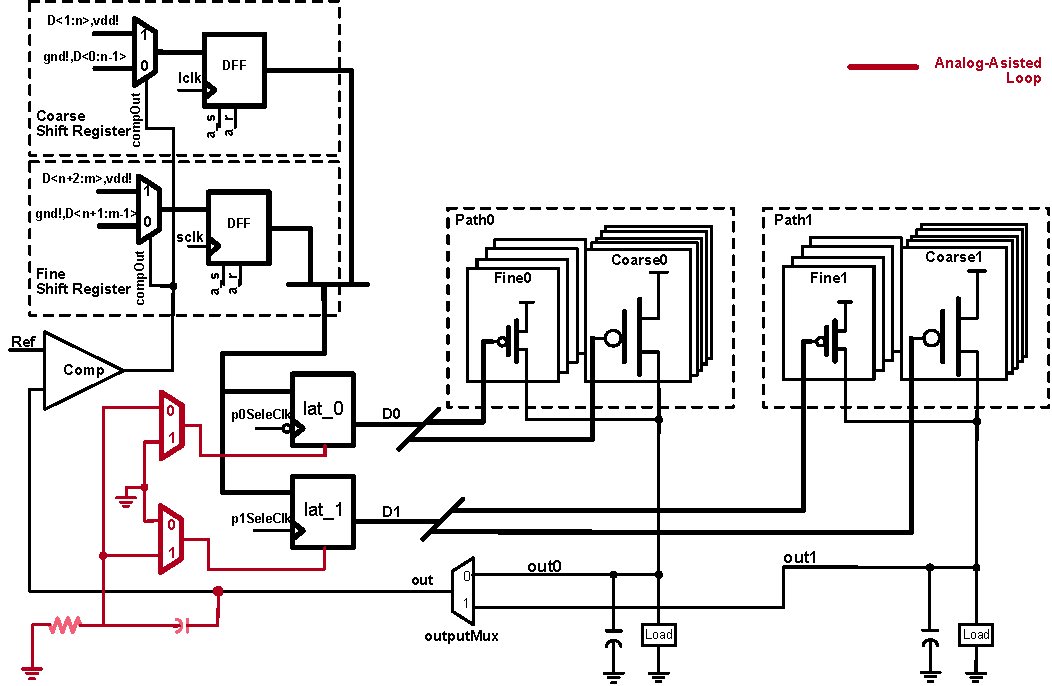
\includegraphics{pic/struc/sche.pdf}
    \caption{Structure of the proposed TDM DLDO}
    \label{fig:diag}
\end{figure*}
\begin{figure}[t!]
    \centering
    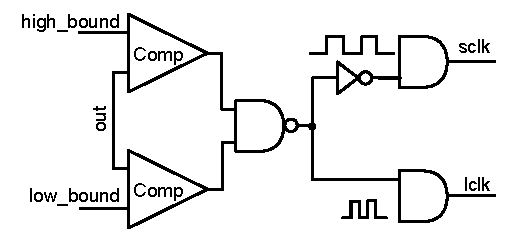
\includegraphics[width=0.7\linewidth]{pic/struc/peak.pdf}
    \caption{Peak detector}
    \label{fig:peak}
\end{figure}
In the TDM scheme design, cross coupling is one of the most salient problems. In the SIMO DC-DC converter proposed in \cite{SIMODCDC}, the sub-converters work in DCM mode, so there is a inherit guard period  between different regulating periods when the current running through the inductor stays zero. And in the TDM micro ring proposed in\cite{wangzhicheng}, a guard period is also inserted between different processing periods to avoid the cross coupling between different outputs. In DLDO, the PMOS arrays are controlled by the shift registers. If we share the shift registers without protection, the states of other PMOS array may be loaded during the switching period and great cross-channel coupling occurs. To solve this problem, we propose the delay switching technique.

Fig.\ref{fig:timing} shows the timing diagram of our design, ``clk'' is the system clock and ``path'' is the path switching signal. The ``sele'' signal generates a pulse at every rising and falling edges of the ``path''. And ``P0/1SeleClk'' are the derivative signal from ``path'' and ``sele'', which drives the latch groups. “D0/1” stands for the states of the PMOS array, and “D” stands for the outputs of the shift register. 

The working principle of the delay switching technique is best interpreted with the reference of the flowchart shown in Fig.\ref{fig:flowchart}. At every switching instance, the ``sele'' signal generates a pulse, in other word, ``sele'' = 1 during this period. If ``path'' = 1 at that time, meaning that the control circuit is to be connected to the power PMOS array 1, then the power PMOS array 0 is latched by ''lat\_0'', so the output voltage at path 0 maintains if the load does not change. Meanwhile, the asynchronous set/reset block load the previously latched states of the array 1 to the shift registers. After all the data are loaded and the pulse at ``sele'' signal disappears, then the power PMOS array 1 is officially connected to the shift registers. And the shift registers starts to control the states of the power PMOS array according to the comparison results until the next switching instance happens. As we load its previous states before we connect one path to the control circuit, no cross-channel coupling should exist.

\subsection{The shared analog-assisted loop}
When the load switch from light to heavy, the power PMOS array may not able to provide enough current, and an undershoot occurs at the output. Normally, the shift register should turn on the PMOS array units to provide more current. However, as is shown in Fig.\ref{fig:aaloop}a, the array unit remains high until the clock arrives and the shift register transfer the comparison result to the array. As a result, the undershoot may be very large in the DLDO. To solve this problem, \cite{AALDO} proposed the analog-assisted loop. The working principle is clear, as is shown in Fig.\ref{fig:aaloop}b, if we can feedback the undershoot to the gate of the array unit, the unit can be at the half-open state before the clock arrive, so the undershoot is greatly reduced. To realize it, an RC loop connect the output and the ground of the inverter buffer. So whenever an undershoot occurs, the buffer can sense it and transfer it to the array instantly.

However, the on-chip capacitors and resisters consume lots of area, but AA loop only takes effect when the load changes, in other word, it stay idle at most of the time. So if we can share the AA loop between different paths, the area efficiency can be further increased. Fig.\ref{fig:sharedAAloop} shows the working principle of the shared AA loop. The high pass network senses the undershoot at the confluent output and transfers it to the $V_{SSB}$ node. 
The multiplexers connected to latch groups are controlled by the ``path'' signal. If one path is selected, the multiplexer connects $V_{SSB}$ to the corresponding latch group and another multiplexer connect GND to the other latch group. So the shared AA loop only take effects on the active path, thus greatly improves the usage efficiency.
\begin{figure}[t!]
    \centering
    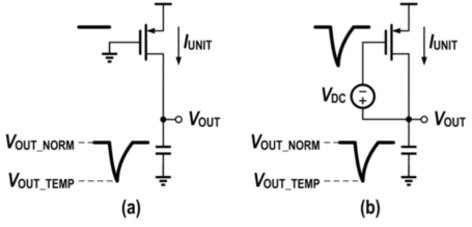
\includegraphics[width=\linewidth]{pic/struc/aaloop.pdf}
    \caption{Comparison between with AA loop and without AA loop}
    \label{fig:aaloop}
\end{figure}
% \begin{figure}[t!]
%     \centering
%     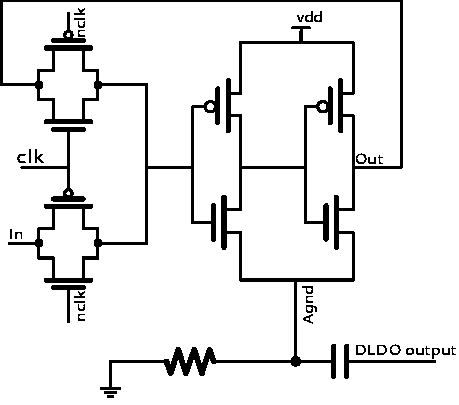
\includegraphics[width=0.9\linewidth]{pic/struc/latch.pdf}
%     \caption{The latch structure appied in ''lat\_0'' and ''lat\_1''}
%     \label{fig:latch}
% \end{figure}
\begin{figure}[t!]
    \centering
    \includegraphics[width=0.9\linewidth]{pic/struc/sharedAAloop.pdf}
    \caption{Shared AA loop}
    \label{fig:sharedAAloop}
\end{figure}
\subsection{Maximum regulated outputs}
In a stable system, the load of the LDO changes at a regular frequency, we can define the load change period as $\rm T_{load}$. Considering the best case that load change happens right after the ``sele'' signal falls down. As is shown in Fig.\ref{fig:sele}, firstly, undershoot (overshoot) occurs, then the shift register alternate the states of the PMOS array to accommodate the load, after the current provided by PMOS array meets the load requirement, the output returns to the regulated voltage. We can define the response time of the DLDO as $\rm T_{response}$, the maximum number of regulated output paths of the TDM DLDO is determined by $\rm T_{load}$, the duration of the ``sele'' signal $\rm T_{sele}$ and the response time $\rm T_{response}$. The maximum regulated outputs are:
\begin{equation}
\rm N \leqslant \frac{\rm T_{load}}{\rm 2\times(T_{sele}+T_{response})}
\end{equation}
The response time of the DLDO is determined by the size of the PMOS array unit, the extent of load variation and clock frequency. Generally a larger PMOS array, smaller load variation and faster clock frequency may reduce the response time. However, larger PMOS array may lead to larger output ripple and a faster clock frequency may increase the dynamic power consumption. The influence of duration of the ``sele'' signal will discussed later. Normally, the response time $\rm T_{response}$ is on the order of tens of clock period.

Note that when the output reaches the nearby of the reference, either turning on or off one PMOS array unit may change the comparison result and limit cycle oscillation (LCO) occurs. In other word, the DLDO only regulate the output at the switching status, and disconnect the PMOS array from the shift register at the stable status may even be beneficial to the performance.
\begin{figure}[t!]
    \centering
    \includegraphics[width=0.9\linewidth]{pic/consid/sele.pdf}
    \caption{The response process of DLDO when load changes}
    \label{fig:sele}
\end{figure}

\section{Circuit implementation and considerations}
\subsection{``sele'' signal duration}
\subsection{R and C selection}
\subsection{Sense amplifier based comparator and D-type flip flop}
Comparator and D-type flip flop are two core circuits in the DLDO design. Comparators are usually sense amplifier based dynamic comparator. The schematic that adopted in our paper is shown in Fig.\ref{fig:comp}. It has two stages, namely pre-amplify stage and regenerate stage. When the clock is low, M4 and M7\~9 turns on, so both ``out+'' and ``out-'' is low. And when the clock switches to high, M8\~9 turns off and M12 turns on, so the pre-amplifier stage amplify the difference at the input nodes. The M1 turns on as well, so the output of the pre-amplifier stage determines the charge speed at ``out+'' and ``out-''. Once one of the nodes reaches the threshold voltage, the regenerate stage forms a positive feedback, and this node become high, the other node become low. D-type flip flop is another structure which plays an important role in the DLDO design, however, the D-type flip flop structure is hardly mentioned in the literature. The D-type flip flop adopted in our design is also a sense amplifier based structure as is shown in Fig.\ref{fig:DFF}, and the working principle of it is similar to the dynamic comparator.  When clock signal is low, M10 is closed,so the sense amplifier stop working, and M1 and M4 charge the nS and nR to high, as a result, the output latch keep the previous input data. When clock signal becomes high, M1 and M4 are closed, and M10 is open, the sense amplifier acts like a positive feedback network, input D and nD transfer the data to the output of the sense amplifier, and the latch keep the result until next clock falling edge arrives. The structure transfer data only at the clock edge, so it works like a D-type flip flop.
\begin{figure}[t!]
    \centering
    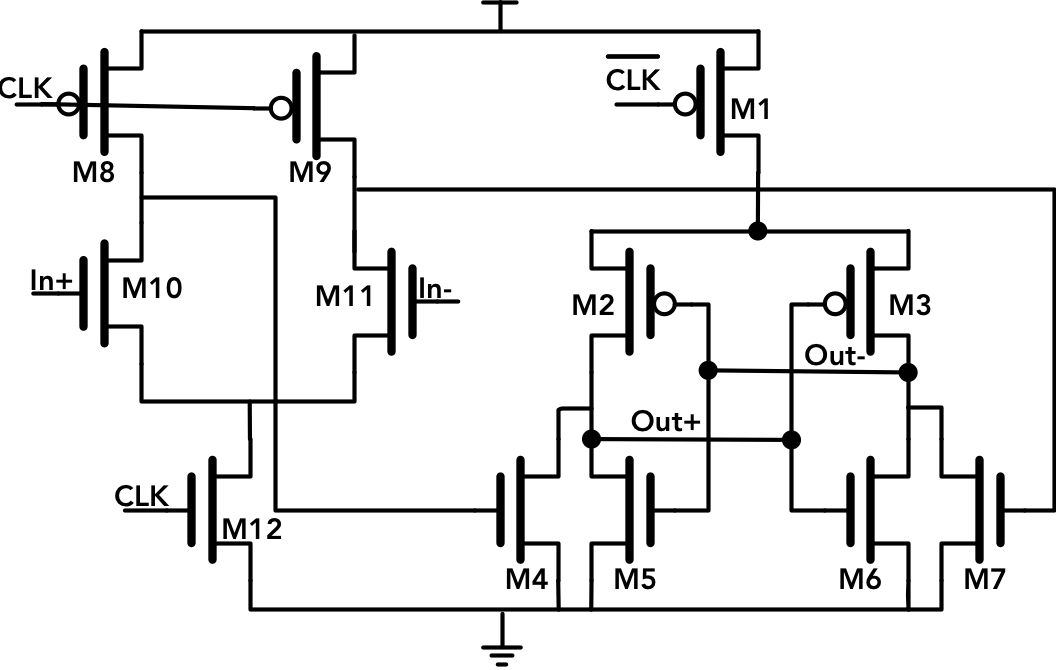
\includegraphics[width=0.9\linewidth]{pic/struc/comp.pdf}
    \caption{Schematic of sense amplifier based dynamic comparator}
    \label{fig:comp}
\end{figure}
\begin{figure}[t!]
    \centering
    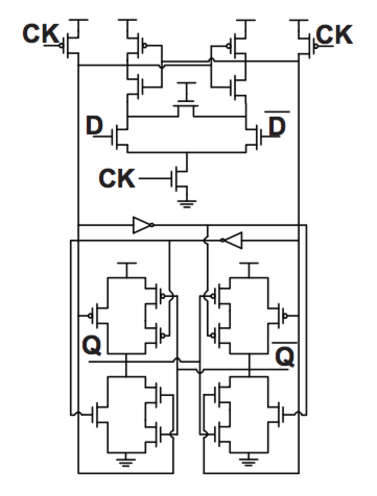
\includegraphics[width=\linewidth]{pic/struc/DFF.pdf}
    \caption{Schematic of sense amplifier based flip flop}
    \label{fig:DFF}
\end{figure}

\section{Measurement results and comparison}
\begin{figure}[t!]
    \centering
    \includegraphics[width=0.9\linewidth]{pic/resu/layout.pdf}
    \caption{The layout of the TDM DLDO}
    \label{fig:layout}
\end{figure}
\begin{figure}[t!]
    \centering
    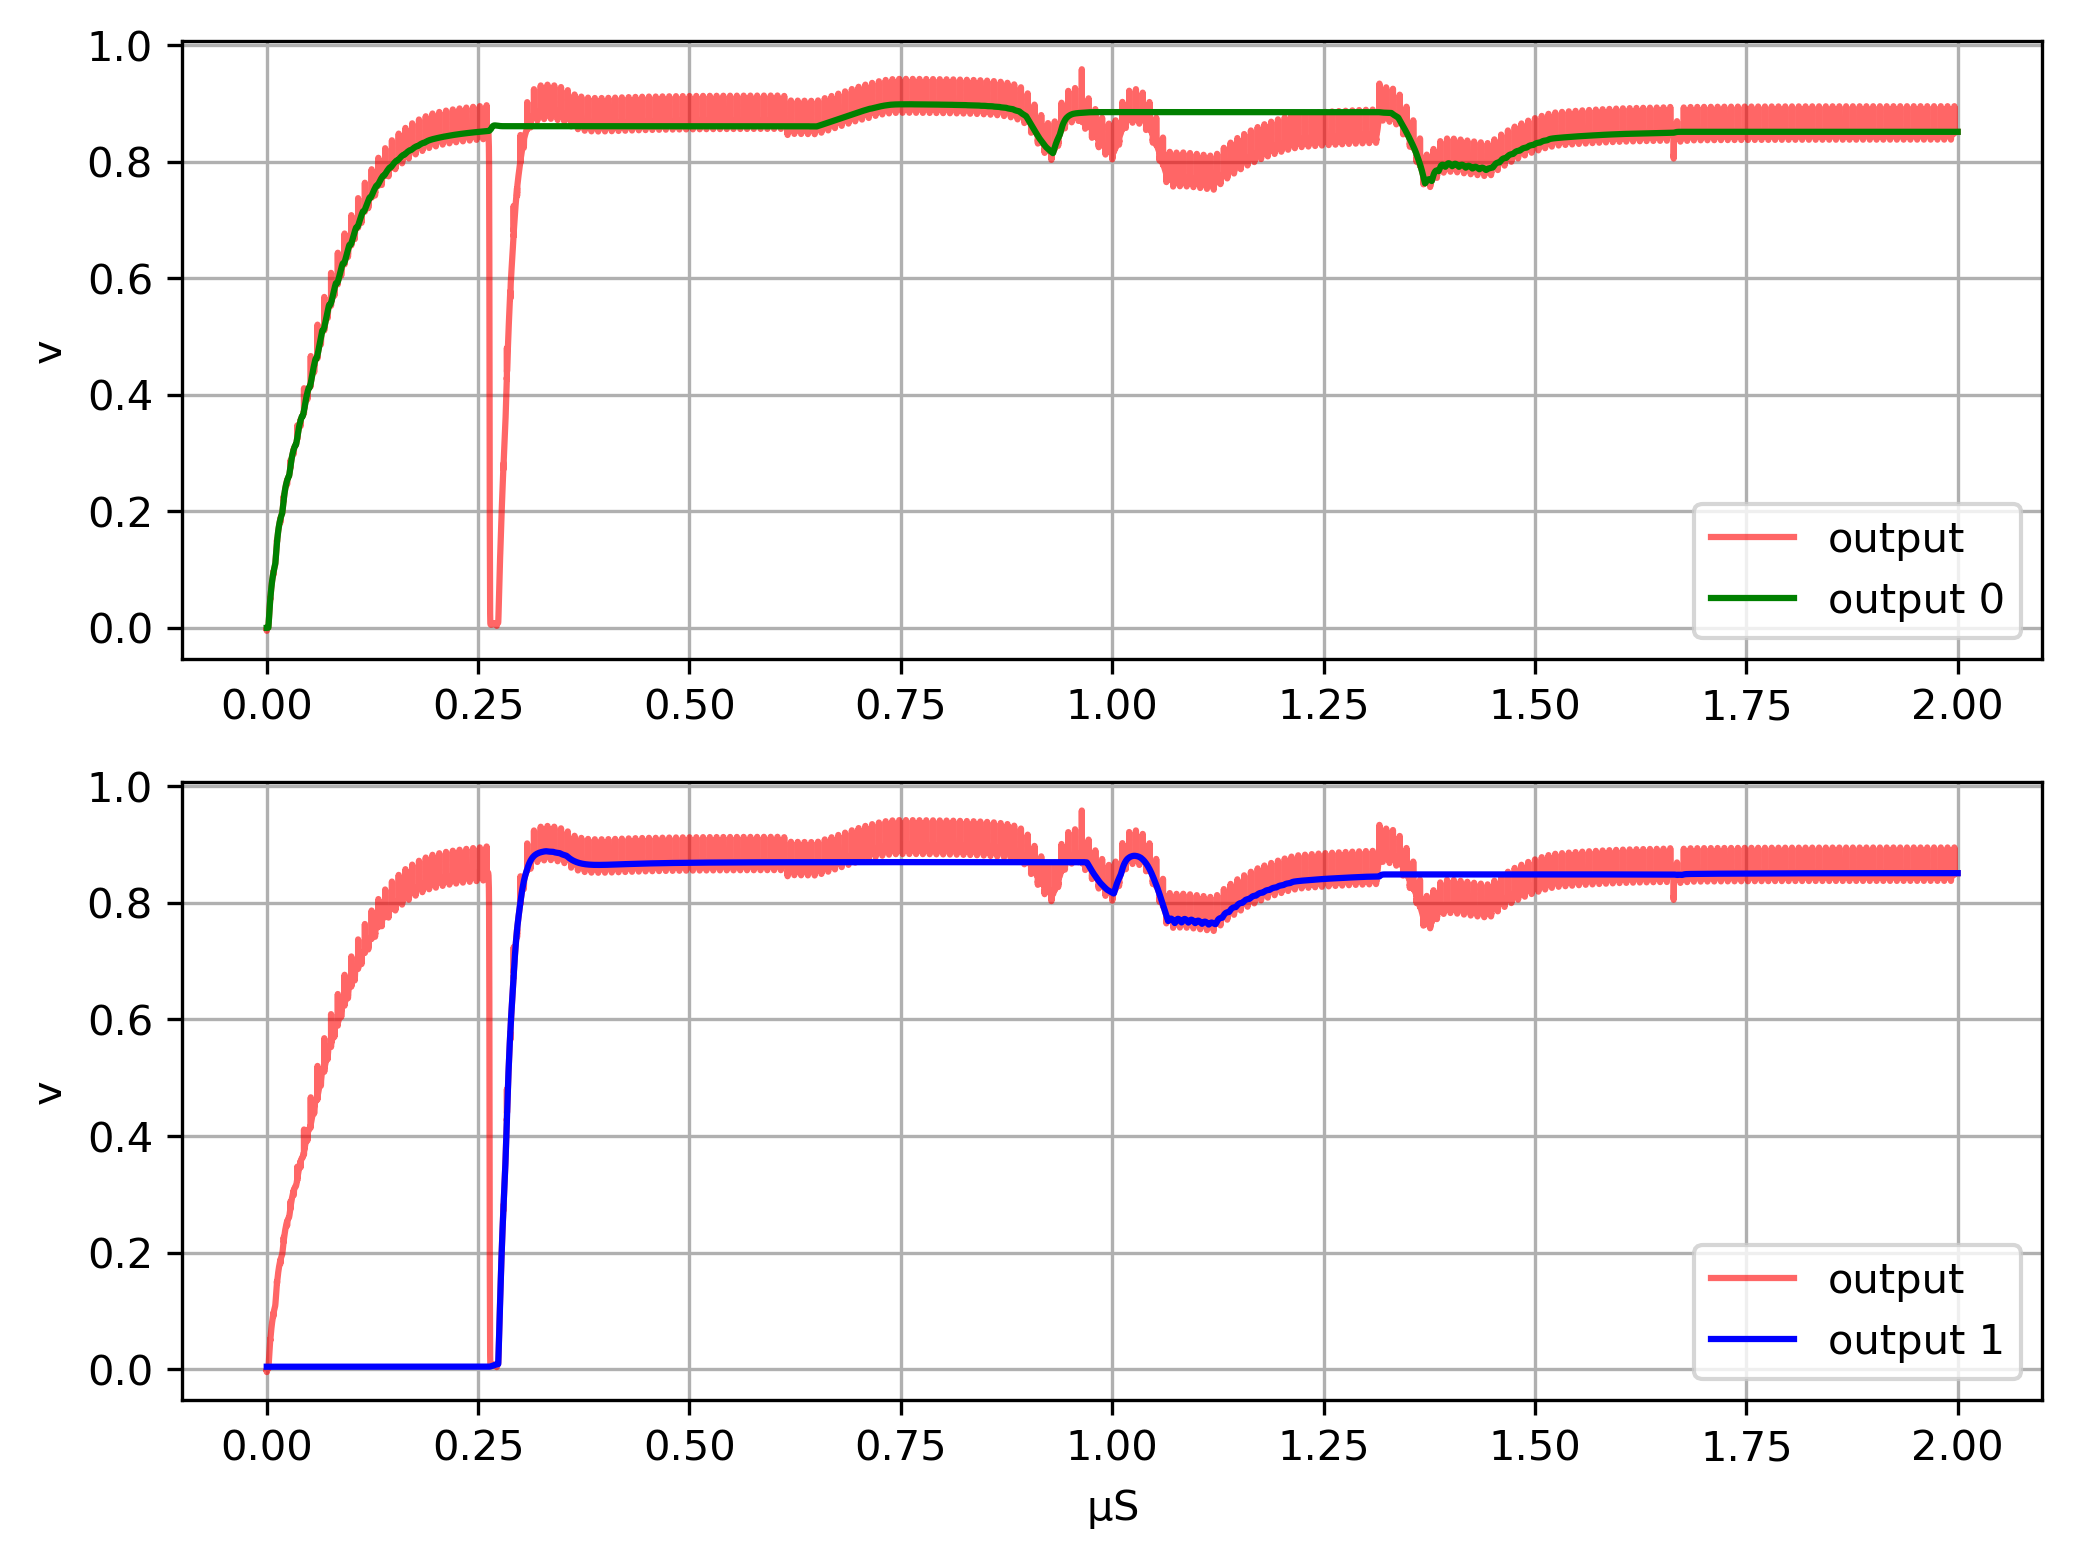
\includegraphics[width=\linewidth]{pic/resu/output.pdf}
    \caption{Output voltage of the proposed TDM DLDO}
    \label{fig:output}
\end{figure}
\begin{figure}[t!]
    \centering
    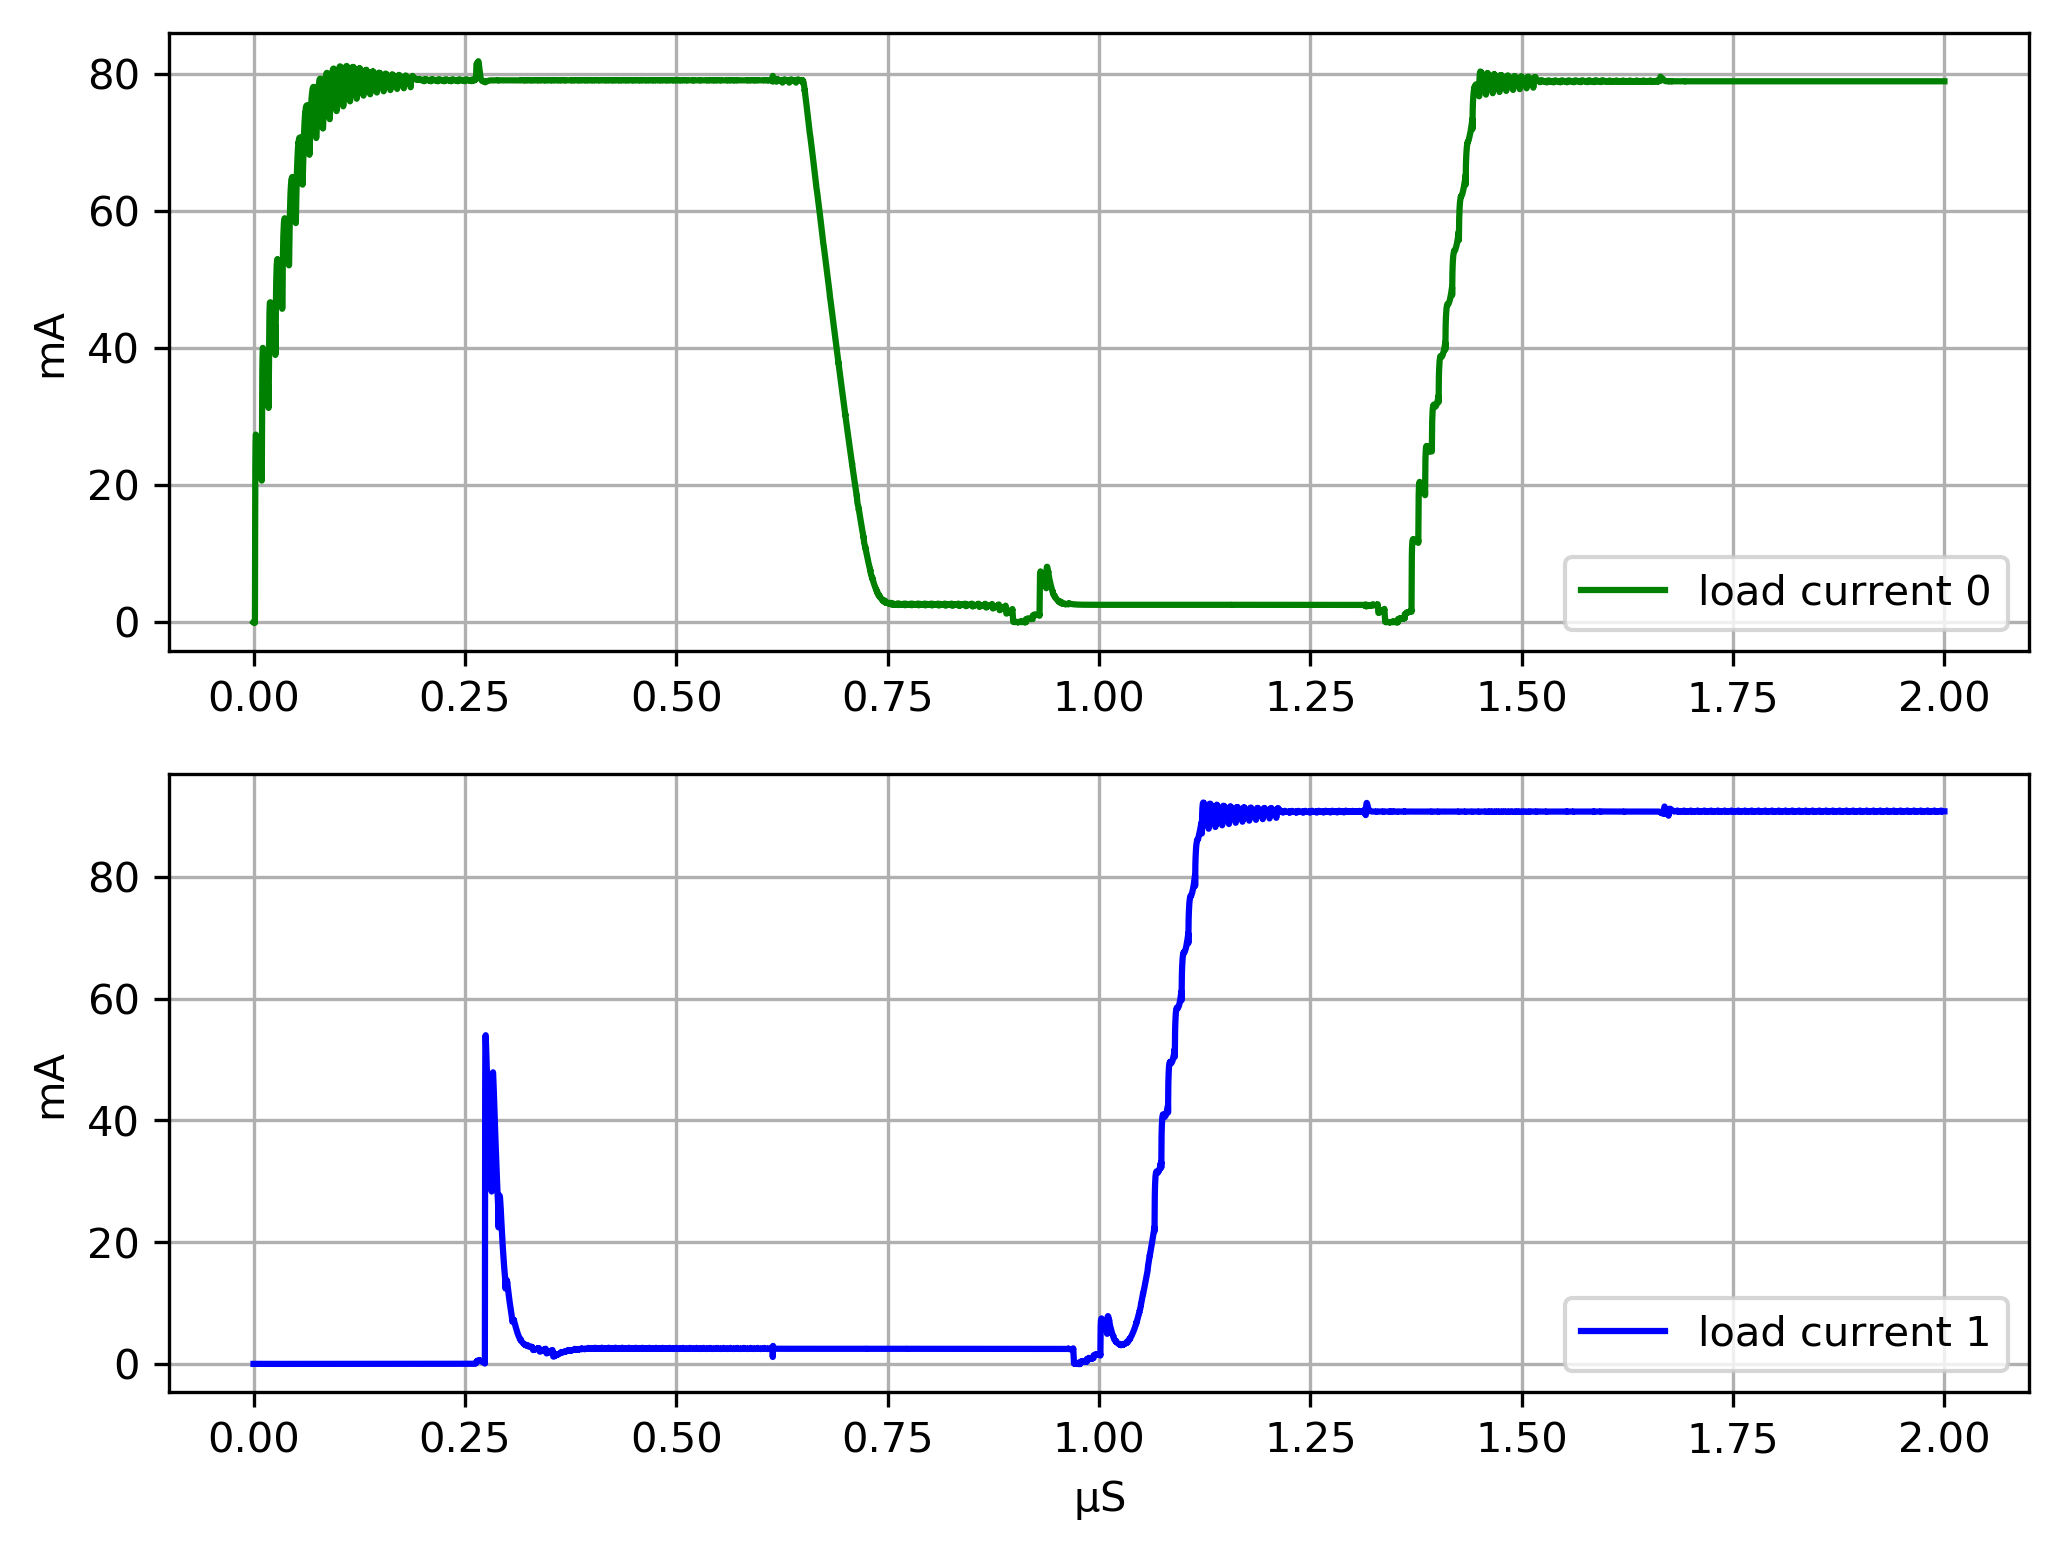
\includegraphics[width=\linewidth]{pic/resu/loadCurr.pdf}
    \caption{Load current of the two paths in TDM DLDO}
    \label{fig:curr}
\end{figure}
\begin{figure}[t!]
    \centering
    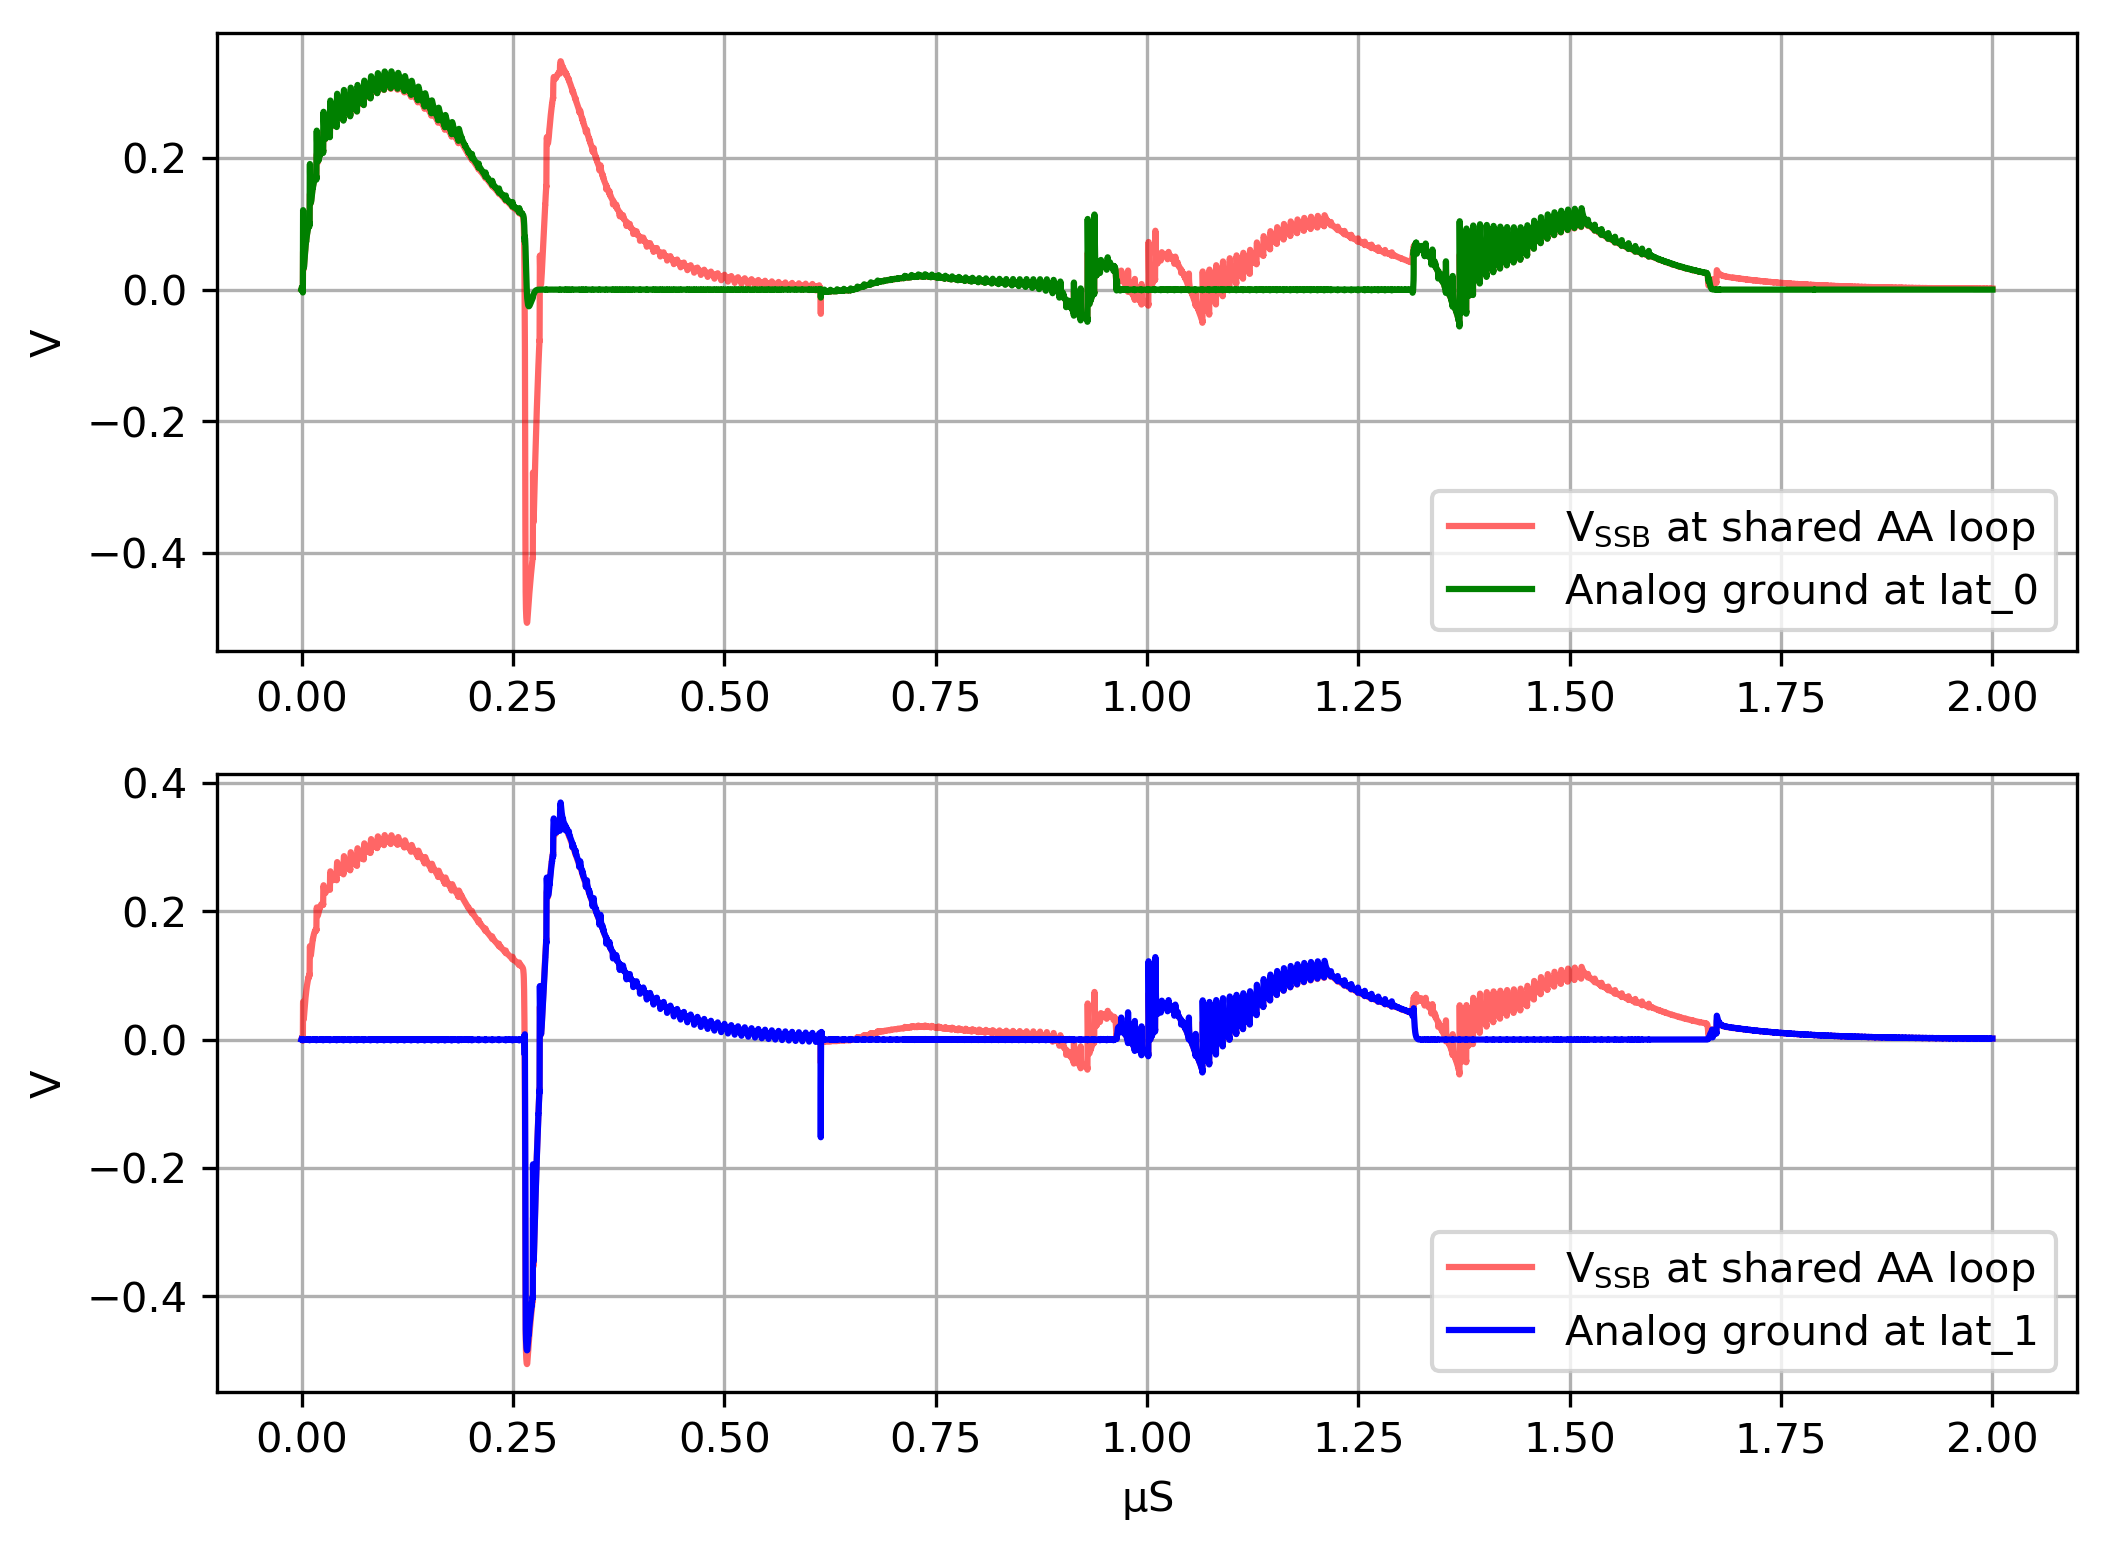
\includegraphics[width=\linewidth]{pic/resu/gnd.pdf}
    \caption{$\rm V_{SSB}$ and analog ground of latch groups}
    \label{fig:gnd}
\end{figure}
\section{Conclusion}

\bibliographystyle{ieeetr}
\bibliography{05ref}
\end{document}


